\documentclass[british,english]{article}
\usepackage[T1]{fontenc}
\usepackage[latin9]{inputenc}
\usepackage{geometry}
\geometry{verbose,tmargin=2cm,bmargin=2cm}
\usepackage{babel}
\usepackage{graphicx}
\usepackage{subcaption}
\usepackage{amsmath}
\usepackage{amsthm}
\usepackage[unicode=true]
 {hyperref}

\makeatletter
%%%%%%%%%%%%%%%%%%%%%%%%%%%%%% Textclass specific LaTeX commands.
\numberwithin{equation}{section}
\numberwithin{figure}{section}

%%%%%%%%%%%%%%%%%%%%%%%%%%%%%% User specified LaTeX commands.
\usepackage{braket}

\@ifundefined{showcaptionsetup}{}{%
 \PassOptionsToPackage{caption=false}{subfig}}
\usepackage{subfig}
\makeatother

\begin{document}

\title{Manual of RyMoP }

\author{Ke Liao\thanks{Any questions or queries should be addressed to \protect\href{mailto:ke.liao.whu@gmail.com}{ke.liao.whu@gmail.com}}}

\maketitle
\tableofcontents{}

\newpage

\section{Introduction}

RyMoPP refers to Rydberg Molecule Potential \foreignlanguage{british}{Program}me
which is written in C++ and developed by Ke Liao for the 5. Physikalisches
Institut, Universit\"at Stuttgart. The programme can calculate the
potential in a Rydberg Molecule using the partial wave scattering
theory, to be precise only S- and P-wave scattering are included.
The programme, though at a primitive stage (no graphic interface or
post-process scripts), includes all the core functions needed to calculate
the S- and P-wave scattering Rydberg Molecule potential. Currently,
the programme has only been tested on Linux (Ubuntu) and Mac OSX with
gcc (g++) compiler 4.8 and it works flawlessly. Older version of gcc
like 4.2 may not support some features and newer versions like gcc
5 abandons some old features so that the programme cannot be compiled.
So choose gcc 4.8 to make life easier.

The programme comes with a compressed file, \emph{RyMoPP.tar.gz},
which when uncompressed will give you 4 folders: \emph{Code, Wave,
Scripts }and \emph{EigenLib}. All of the essential codes are stored
in \emph{Code}, \emph{EigenLib }is the \href{http://eigen.tuxfamily.org/index.php?title=Main_Page}{Eigen Library},
\emph{Scripts }contains some pre- and post-processing scripts and
\emph{Wave }contains a selected range of wave functions that you can
use. If you want to use more wave functions, you have to copy the
corresponding files into this folder. One important thing to note
is that the names of the newly copied files have to have the same
format as the old ones which are already there. Originally I obtain
those wave function files by converting the {*}.mat files to {*}.txt
files. I wrote a script called \emph{convert.py} to do this job. I
will address more about this script later in Scripts \ref{subsec:Scripts}. 

For record, I list the essential files here and explain briefly what
they do. 

\paragraph{Core Files}
\begin{enumerate}
\item \emph{Kore.cpp}, which is the core file in this programme and contains
all the essential functions;
\item \emph{specfunc.h}, which contains a collection of special functions,
including the Spherical Harmonics and another Spherical Harmonics
without $\sin\theta$\footnote{I will introduce this function in detail. It is crucial to the P-wave
scattering calculation.}. Though it is not included directly in Kore.cpp, it is contained
in 'integral.h';
\item \emph{memalloc.h}, which handles memory allocation. It is used in
'integral.h';
\item \emph{integral.h}, which provides integration of 3D angular integration.
In this file, it includes 'memalloc.h' and 'specfunc.h'. 
\item \emph{line.h}, which provides the functions used in 'Kore.cpp' to
read data files correctly.
\item \emph{compile.sh}, which is used to compile the programme. In this
file, it compiles the Kore.cpp with the option linked to the 'EigenLib'
library, which handles the matrices manipulations.
\end{enumerate}
%

\paragraph{Scripts\label{subsec:Scripts}}

Above 5 files are the essential ones. During the process, I also wrote
two python scripts, which are 
\begin{enumerate}
\item convert.py, which can convert the wave function files from {*}.mat
format to {*}.txt format, and the latter is the format that this programme
can read. Users have to pay attention to the format of the files'
name and the files themselves. The converted wave function files have
the eigen energy of this state at the end of the file.
\item get\_pot.py, which is the post-processing script to get data from
the output files from the main programme.
\end{enumerate}
%
The implementation of the code involves some theoretical derivations,
so the next section is dedicated to the basics of the theory. After
that, I will dive into the details of the codes. In the end, some
examples will be shown.

\section{Theoretical Basis}

In this section, we go through the basics of the theory. The system
under consideration is a Rydberg molecule, which consists of a Rydberg
atom and a ground state atom sitting in the range of the former. Due
to the scattering between the Rydberg electron and the ground state
atom, an effective attraction between these two atoms can form. Our
goal is to calculate the effective potential between the Rydberg atom
and the ground state atom when the distances between them changes.
The distance here refers to the distance between the ground state
atom and the nucleus of the Rydberg atom. The general idea is to expand
the scattered electronic wave function with the unperturbed eigenfunctions
from the isolated Rydberg atom, based on the linear variational principle,
we can get the perturbed electronic wave function and energy, in turn,
the energy of the electron acts as an effective potential for the
ground state atom in a wave similar to the Born-Oppenheimer approximation
in solids. 

\subsection{Atomic Wave Functions}

First of all, we need the unperturbed wave functions of a isolated
atom to be the basis functions. Consider the Schr\"odinger equation
for a Rydberg atom: 

\begin{equation}
\left[\frac{{\bf p}^{2}}{2m_{e}}+V_{mod}(r)\right]\Ket{\Psi}=E\Ket{\Psi},
\end{equation}
where $V_{mod}(r)$ is a effective potential and we split the wave
function into radial and angular part
\begin{equation}
\Psi(r,\theta,\phi)=R({\bf r})\tilde{Y}(\theta,\phi).
\label{equ:wavefun}
\end{equation}
In the internal wiki of Pi5, there is a detailed explanation about
how to get the radial part of the wave function, so we will skip this
part here. But we have to point out that the final calculated result
in the wave function file is only the radial part and it is not directly
stored as $r$ and $R(r)$, instead a transform of the variables is
used:

\begin{equation}
\begin{aligned}
x&=\sqrt{r},\\
X(x)&=x^{3/2}R(r).
\label{equ:trans}
\end{aligned}
\end{equation}As for the angular part, since we take the spin orbital interaction
into account, spinors, which are the combinations of two spherical
harmonics, should be used here.

\begin{equation}
\begin{aligned}
\tilde{Y}_{(j-\frac{1}{2},\frac{1}{2})j m_{j}}&=\left(\sqrt{\frac{j+m_{j}}{2j}}Y_{j-\frac{1}{2},m_{j}-\frac 12}, \sqrt{\frac{j-m_{j}}{2j}}Y_{j-\frac 12,m_{j}+\frac 12}\right),\\
\tilde{Y}_{(j+\frac{1}{2},\frac{1}{2})jm_{j}}&=\left(-\sqrt{\frac{j-m_{j}+1}{2j+2}}Y_{j+\frac{1}{2},m_{j}-\frac 12}, \sqrt{\frac{j+m_{j}+1}{2j+2}}Y_{j+\frac 12,m_{j}+\frac 12}\right),
\label{equ:spinors}
\end{aligned}
\end{equation}
where $ {\bf j} = {\bf l} + {\bf s}$, and $m_{j} = -|l-s|,-|l-s|+1,\dots,|l+s|-1,|l+s|$. Note that in practice we can use the relation between $m_j$ and $m$: $m=m_j-\frac {1}{2}$ and $m+1 = m_j + \frac{1}{2}$. For detailed information please refer to this book.\cite{Biedenharn1981}
\subsection{Pseudopotential in Molecular Hamiltonian}

For a highly excited Rydberg atom interacting with a ground state
atom, the Hamiltonian is

\begin{equation}
H=\frac{{\bf P}^{2}}{M}+H_{el}+V_{n,e}({\bf r,R})
\end{equation}
where $H_{el}$ is the atomic Hamiltonian we mentioned in last subsection,
$M$ is the mass of the atom, ${\bf P}$ and ${\bf R}$ are the relative
momentum and position of the ground state atom with respect to the
ionic core of the Rydberg atom respectively and ${\bf r}$ is the
relative position of the Rydberg electron to the ionic core. $V_{n,e}({\bf r,R})$
is the famous Fermi-Pseudopotential:

\begin{equation}
V_{n,e}({\bf r,R})=2\pi A_{s}[k(R)]\delta({\bf r}-{\bf R})+6\pi A_{p}^{3}[k(R)\overleftarrow{]\nabla}\delta({\bf r}-{\bf R})\overrightarrow{\nabla}
\end{equation}
where $A_{s}(k)=-\tan[\delta_{0}(k)]/k$ and $A_{p}^{3}(k)=-\tan[\delta_{1}(k)]/k^{3}$
denote the energy-dependent triplet s- and p-wave scattering lengths.
It is worth pointing out that $\delta_{l=0,1}(k)$ are the energy
dependent phase shifts and $\frac{k(R)^{2}}{2}=E_{kin}=-\frac{1}{2}n^{*2}+\frac{1}{R}$
where $n^{*}$ is the effective principal quantum number.

 Unfortunately, we do not have analytical expressions for $\delta_{l=0,1}(k)$ , so
we have to do a fitting based on the data we have got. See figure
(\ref{fig:fitting} ) for an example of $N=35$. This also means that for each $N$ we should do a fitting of the scattering length. Another less troublesome way would be fitting the phase shift with respect to $k$, but as I tried it is not so good (anyway the users are encouraged to use any methods that are better).
%%%%%%%%%%%%%%%%%%%%%%%%%%%%%%%%%%%%%%%%%%%%%%%%%%%%%%%%%%
\begin{figure}
\centering
\begin{subfigure}[h]{0.45\linewidth}
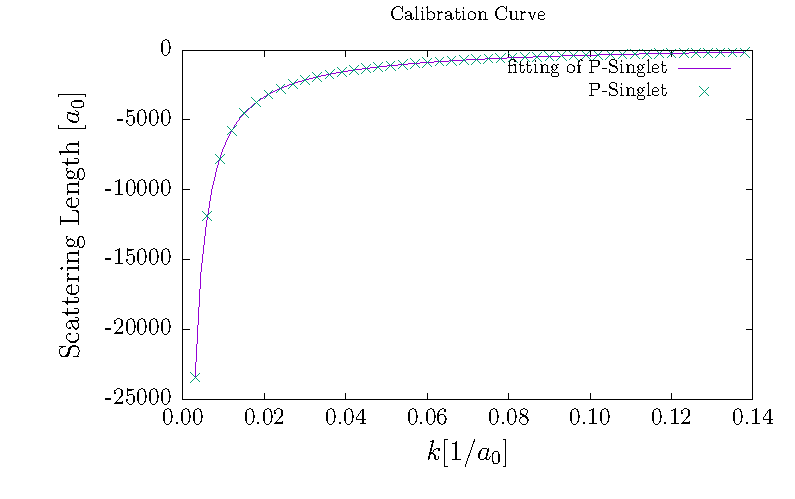
\includegraphics[width=\textwidth]{../Figs/PSinglet}
\end{subfigure}
\begin{subfigure}[h]{0.45\linewidth}
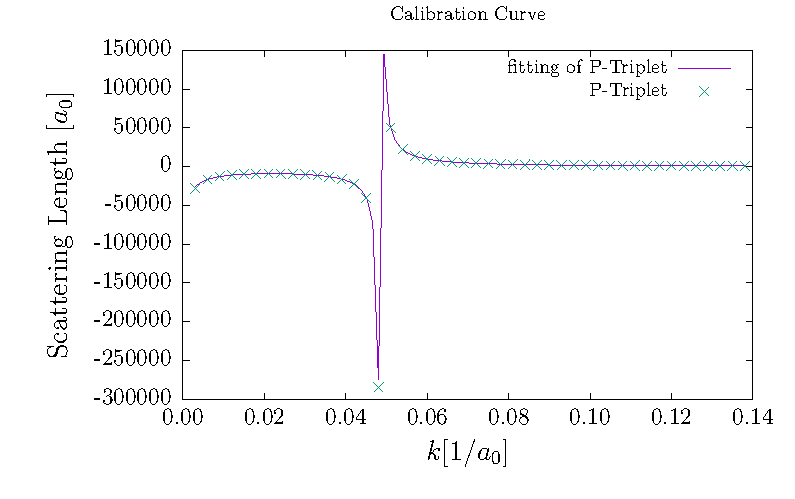
\includegraphics[width=\textwidth]{../Figs/PTriplet}
\end{subfigure}
\caption{
\label{fig:fitting}
~
}
\end{figure}
%%%%%%%%%%%%%%%%%%%%%%%%%%%%%%%%%%%%%%%%%%%%%%%%%%%%%%%%%

The matrix elements can be calculated by sandwiching the full Hamiltonian with the basis functions
\begin{equation}
H_{ij}=\braket{\Psi_i|H_0+V_{n,e}|\Psi_j}=H_{0_{ij}}+V_{ij},
\end{equation}
where $H_0 =\frac{{\bf P}^{2}}{M}+H_{el}$. $H_0$ is a diagonal matrix whose diagonal entries are the eigen energies of the original atomic states. In the following subsections, we are going to discuss how to calculate $V_{ij}$.
\subsection{S-wave scattering}
To include the singlet and triplet states in our calculations \cite{}, we use a slightly different Hamiltonian than the one we showed above
\begin{equation}
\hat H({\bf r, Z})=\hat H_0+\sum_{i=S,T}2\pi A^i_S({\bf k})\delta^3({\bf r}-Z\hat z)\hat I_i+\sum_{i=S,T}6\pi A_P^i({\bf k})\delta^3({\bf r}-Z\hat z)\overleftarrow{\nabla}\cdot\overrightarrow\nabla\hat I_i+A\hat S_2\cdot \hat I_2,
\end{equation}
 where $\hat I_T=\hat S_1\cdot \hat S_2+\frac 34$ is the triplet operator, when applied to triplet state, the eigenvalue is 1, otherwise is 0, vise versa for $\hat I_S$ which is the singlet operator.

First, let's focus on the calculations involving the angular part of the wave function. In calculations we assume that the ground atom is always spin up which is represented by the second uparrow in following formulae, which is viable in experiments. So we shall have:
\begin{equation}
	\begin{aligned}
	\hat I_T\ket{\uparrow\uparrow}&=1\ket{\uparrow\uparrow},\\
	\hat I_T\ket{\downarrow\downarrow}&=1\ket{\downarrow\downarrow},\\
	\ket{\downarrow\uparrow}&=\frac{1}{\sqrt{2}}\left[\frac{1}{\sqrt{2}}(\ket{\uparrow\downarrow}+\ket{\downarrow\uparrow})-\frac{1}{\sqrt{2}}(\ket{\uparrow\downarrow}-\ket{\downarrow\uparrow})\right],\\
	\hat I_T\ket{\downarrow\uparrow}&=\frac{1}{2}(\ket{\uparrow\downarrow}+\ket{\downarrow\uparrow}),\\
	\hat I_S\ket{\downarrow\uparrow}&=-\frac{1}{2}(\ket{\uparrow\downarrow}-\ket{\downarrow\uparrow}).
	\end{aligned}
\end{equation}
As we have showed in equ (\ref{equ:spinors}), every spinor has two components which can be symbolised as $\tilde Y=(\uparrow,\downarrow)$. So the total wave function, the one of the Rydberg electron and the one of the electron from the ground state atom, is
\begin{equation} 
\begin{aligned}
Y\otimes G&=(\ket{\uparrow},\ket{\downarrow})\otimes \ket{\uparrow}\\
	  &=\left(\ket{\uparrow\uparrow},\ket{\downarrow\uparrow}\right).
\end{aligned}
\end{equation}
Notice that the 3D $\delta^3({\bf r})$ has the following form in integrations:
\begin{equation}
\int \mathrm d^3 r \delta(\vec r -\vec R)=\iiint\delta(r-R)\delta(\theta-\theta_0)\delta(\varphi-\varphi_0)\frac{1}{r^2\sin(\theta)}.
\end{equation}
Using the orthogonality between the spin up $\bra{\uparrow}$ and spin down $\ket{\downarrow}$ states of the ground state atom, the calculations go straightforward
\begin{equation}
\begin{aligned}
&\int \mathrm d {\bf r}R^*_i({\bf r})(\bra{\uparrow\uparrow}',\bra{\downarrow\uparrow}')\sum_{i=S,T}2\pi A^i_S(k)\delta^3({\bf r}-Z\hat z)\hat I_i(\ket{\uparrow\uparrow},\ket{\downarrow\uparrow})R_j({\bf r})\\
&=2\pi \int \delta(r-Z) R^*_i(r)R_j(r)\mathrm d r\left[A_S^T\left.\braket{\uparrow'\uparrow'|\uparrow\uparrow}\right|_{\theta=0,\varphi=0}+\frac 12 \left.\braket{\downarrow'\uparrow'|\downarrow\uparrow}\right|_{\theta=0,\varphi=0}(A_S^S+A_S^T)\right]
\end{aligned}
\label{equ:angularS}
\end{equation}
Now let's finish the calculations involving the radial part of the wave functions. The singlet and triplet operators only influence the calculations of the angular part. So we can continue the calculations based on the result we got in equ (\ref{equ:angularS}), neglect the angular part for now and  notice the changing of variables we mentioned in equ (\ref{equ:trans}),
\begin{equation}
\begin{aligned}
&\int_0^{\infty} 2\pi R^*_i( r)\delta(r - Z)R_j(r)\mathrm dr\\
&= 2\pi \int_0^{\infty} X^*_i(x)x^{-\frac{3}{2}}\delta(x^2-Z)X_j(x)x^{-\frac{3}{2}}2x\mathrm dx\\
&= 2\pi X_i^*(\sqrt{Z})X_j(\sqrt{Z})Z^{-\frac{3}{2}}
\end{aligned}
\end{equation}
In the end, we multiply the radial and angular contributions to get the final result. An important and interesting fact about spherical harmonics is that at $\theta=0, \varphi=0$, only those with $m=0$ have non-zero contributions. So when we construct the matrix, we can use this fact and substantially reduce the amount of computational resource. This is how we are going to construct the off-diagonal entries for the S-wave scattering Hamiltonian matrix.

\subsection{P-wave Scattering}
The calculations for P-wave scattering are a bit tricky, since they involve the calculations of ${\bf \nabla}$ in spherical coordinate system. In the P-wave scattering potential, 
\begin{equation}
\hat{V}_p = 6\pi A_{p}^{3}[k(R)]\overleftarrow{\nabla}\delta({\bf r}-{\bf R})\overrightarrow{\nabla},
\end{equation} 
where $overleftarrow{\nabla}$ means that the operator acts on the bra $\bra{}$ from the left and vice versa for $\overrightarrow{\nabla}$. In spherical coordinate system, 
\begin{equation}
\begin{aligned}
{\bf \nabla}={\frac{\partial f}{\partial r}}\hat{\mathbf r}
+ {\frac{1}{r}}{\frac{\partial f}{\partial \theta}}\hat{\boldsymbol \theta}
+ {\frac{1}{r}\sin\theta}{\frac{\partial f}{\partial \varphi}}\hat{\boldsymbol \varphi}.
\end{aligned}
\end{equation}
When we apply the P-wave scattering potential operator to the wave function (\ref{equ:wavefunc}), we get 
\begin{equation}
\begin{aligned}
& <\Psi|\nabla\delta({\bf r}-Z{\hat z})\nabla|\Psi'>\\
&= \int\mathrm d^3r\nabla\Psi^*\delta({\bf r}-Z{\hat z})\nabla \Psi \\
&= \iiint \delta(r-R)\delta(\theta-\theta_0)\delta(\varphi-\varphi_0)\frac{1}{r^2\sin(\theta)}\left[\tilde{Y}^*(\theta,\varphi)\tilde{Y}'(\theta,\varphi)\frac{\partial R^*(r)}{\partial r}\frac{\partial R'(r)}{\partial r}\right.\\
&\left.+\frac{R^*(r)}{r}\frac{R'(r)}{r}\frac{\partial \tilde{Y}^*(\theta,\varphi)}{\partial \theta}\frac{\partial \tilde{Y}'(\theta,\varphi)}{\partial \theta}+\frac{\partial \tilde{Y}^*(\theta,\varphi)}{\partial \varphi}\frac{\partial \tilde{Y}'(\theta,\varphi)}{\partial \varphi}\frac{R^*(r)}{r\sin(\theta)}\frac{R'(r)}{r\sin(\theta)}\right]r^2\sin(\theta)\mathrm d r \mathrm d \theta \mathrm d\varphi \\
&=\left[\tilde{Y}^*(\theta,\beta)\tilde{Y}'(\theta,\beta)\right]_{\theta=0,\beta=0}\left[\frac{\partial R^*(r)}{\partial r}\frac{\partial R'(r)}{\partial r}\right]_{r=Z}+\left[\frac{\partial \tilde{Y}^*(\theta,\varphi)}{\partial \theta}\frac{\partial \tilde{Y}'(\theta,\varphi)}{\partial \theta}\right]_{\theta=0,\varphi=0}\left[\frac{R^*(r)}{r}\frac{R'(r)}{r}\right]_{r=Z}\\
&+\left[\frac{1}{\sin^2(\theta)}\frac{\partial \tilde{Y}^*(\theta,\varphi)}{\partial \varphi}\frac{\partial \tilde{Y}'(\theta,\varphi)}{\partial \varphi}\right]_{\theta=0,\varphi=0}\left[\frac{R(r)R'(r)}{r^2}\right]_{r=Z}.
\end{aligned}
\end{equation}
For clarity let us denote the three terms in the final result into separate names,
\begin{align}
PWS1&=\left[\tilde{Y}^*(\theta,\beta)\tilde{Y}'(\theta,\beta)\right]_{\theta=0,\beta=0}\left[\frac{\partial R^*(r)}{\partial r}\frac{\partial R'(r)}{\partial r}\right]_{r=Z},\\
PWS2&=\left[\frac{\partial \tilde{Y}^*(\theta,\varphi)}{\partial \theta}\frac{\partial \tilde{Y}'(\theta,\varphi)}{\partial \theta}\right]_{\theta=0,\varphi=0}\left[\frac{R^*(r)}{r}\frac{R'(r)}{r}\right]_{r=Z},\\
PWS3&=\left[\frac{1}{\sin^2(\theta)}\frac{\partial \tilde{Y}^*(\theta,\varphi)}{\partial \varphi}\frac{\partial \tilde{Y}'(\theta,\varphi)}{\partial \varphi}\right]_{\theta=0,\varphi=0}\left[\frac{R(r)R'(r)}{r^2}\right]_{r=Z}.
\end{align}
The $PWS3$ is the most difficult one to calculate because of the singularity at $\theta=0$ brought by $\frac{1}{\sin^2 \theta}$. For $PWS1$, we can reuse the calculations from S-wave scattering for the angular part and as for the radial part we use differences to approximate the derivatives; for $PWS2$, the following formula is helpful:
\begin{equation}
\frac{\partial Y_l^m(\theta,\varphi)}{\partial \theta}= m\cot \theta Y^m_l(\theta,\varphi) + \frac{\sqrt{\Gamma(l-m+1)\Gamma(l+m+2)}}{\sqrt{\Gamma(l+m+1)\Gamma(l-m)}}e^{-i\varphi}Y^{m+1}_l(\theta,\varphi).
\label{equ:der_theta}
\end{equation}
A scrutinization on formula (\ref{equ:der_theta}) will tell us that $\left.\frac{\partial Y_l^m(\theta,\varphi)}{\partial \theta}\right|_{\theta=0,\varphi=0}=0$, because
\begin{itemize}
\item when $m=0$, the first term is zero and so is the second term since $Y_l^1(0,0)=0$,
\item when $m\neq0$, $Y_l^{m\neq0}(0,0)=0$.
\end{itemize}
However, for possible future adaption of the code, we keep the general calculation of the derivative with respect to $\theta$ of the spherical harmonics instead of setting directly $PWS2=0$. 

Now let's focus on $PWS3$. To start with, ignore the radial part first and use the formula
\begin{equation}
\frac{\partial Y^m_l}{\partial \varphi}=imY^m_l,
\end{equation}
where $i$ is the imaginary unit. In the spinor spherical harmonics, we will adopt $l,m$ notation instead of $j,m_j$ notation here just for convenience. 
\begin{equation}
\begin{aligned}
&\left[\frac{1}{\sin^2\theta}\left(\frac{\partial \tilde{Y}_j^{m_j}}{\partial \varphi}\right)^* \left(\frac{\partial \tilde{Y}_{j'}^{m_j'}}{\partial \varphi}\right)\right]_{\theta=0,\varphi=0}\\
&=\left[\frac{1}{\sin^2\theta} \begin{pmatrix} \frac{\alpha\partial Y_l^{m}}{\partial \varphi},&\frac{\beta\partial Y_l^{m+1}}{\partial \varphi}\end{pmatrix}^*\begin{pmatrix} \frac{\alpha'\partial Y_{l'}^{m'}}{\partial \varphi} &\\
\frac{\beta' \partial Y_{l'}^{m'+1}}{\partial \varphi} &
\end{pmatrix}\right]_{\theta=0,\varphi=0}\\
&=\left[\frac{1}{\sin^2\theta} \begin{pmatrix} \alpha i m Y_l^{m},&\beta i(m+1)Y_l^{m+1}\end{pmatrix}^*\begin{pmatrix} \alpha'im' Y_{l'}^{m'} &\\
\beta' i(m'+1) Y_{l'}^{m'+1} &
\end{pmatrix}\right]_{\theta=0,\varphi=0}\\
&=\frac{1}{\sin^2\theta}\left[\alpha\alpha'mm'Y_l^{m*} Y_{l'}^{m'}+\beta\beta'(m+1)(m'+1)Y_{l}^{m+1*}Y_{l'}^{m'+1}\right]_{\theta=0,\varphi=0}.
\end{aligned}
\label{equ:pws3}
\end{equation}
When we get this result, it is time to look into the expression of spherical harmonics
\begin{equation}
Y_{l }^{m}(\theta ,\varphi )=(-1)^{m}{\sqrt {{(2l +1) \over 4\pi }{(l -m)! \over (l +m)!}}}\,P_{l }^{m}(\cos {\theta })\,e^{im\varphi },
\end{equation} 
where the Associated Legendre polynomials are
\begin{equation}
P_{l }^{m}(\cos \theta )=(-1)^{m}(\sin \theta )^{m}\ {\frac {d^{m}}{d(\cos \theta )^{m}}}\left(P_{l }(\cos \theta )\right)\,
\end{equation}
where $P_l$ is the Legendre polynomials. We can stop here because we only need to know the order of $\sin \theta$ in the spherical harmonics and we know it from the above expression that it is $m$. To cancel out the $1/\sin ^2 \theta$ in equation (\ref{equ:pws3}) and obtain a finite value, we need
\begin{equation} 
|m|+|m'|=2 \text{ or } |m+1|+|m'+1|=2.
\end{equation}
 In practice, we set $PWS3=0$ when the above condition is not met, and when it is met we need a special way to calculate it. We define a new kind of spherical harmonics which is called \emph{Spherical Harmonics without $\sin \theta$($YNoSin_l^m$)}, for example
\begin{equation}
\begin{aligned}
Y_{3}^{1}(\theta ,\varphi )&={-1 \over 8}{\sqrt {21 \over \pi }}\cdot e^{i\varphi }\cdot \sin \theta \cdot (5\cos ^{2}\theta -1),\\
YNoSin_{3}^{1}(\theta ,\varphi )&={-1 \over 8}{\sqrt {21 \over \pi }}\cdot e^{i\varphi }\cdot (5\cos ^{2}\theta -1).
\end{aligned}
\end{equation}
So basically we manually cancel out the $\sin \theta$'s by using $YNoSin_l^m$'s instead of $Y_l^m$'s when the condition is met. The final expression for $PWS3$ is
\begin{equation}
PWS3=
\begin{cases}
   \left[\alpha\alpha'mm'YNoSin_l^{m*} YNoSin_{l'}^{m'}\right.\\
   +\left.\beta\beta'(m+1)(m'+1)YNoSin_{l}^{m+1*}YNoSin_{l'}^{m'+1}\right]_{\theta=0,\varphi=0} ,& \text{if } |m|+|m'|=2 \text{ or } |m+1|+|m'+1|=2\\
    0,              & \text{otherwise}
\end{cases}
\end{equation}
\section{Results}
A data file named data702.txt contains a latest run with 702 basis functions, including the P Wave scattering. To be continued... 
Some other literatures\cite{Anderson2014,Biedenharn1981,Balewski2014,Bendkowsky2009,Kurz2013,Bendkowsky2010}
\bibliography{bib}
\bibliographystyle{unsrt}
\end{document}
